\documentclass{article}
\usepackage[utf8]{inputenc}

\usepackage[T1]{fontenc}
\usepackage{amssymb}
\usepackage[swedish]{babel}
\usepackage{amsmath}
\usepackage{lmodern}
\usepackage{units}
\usepackage{icomma}
\usepackage{color}
\usepackage{graphicx}
\usepackage{bbm}
\usepackage{hyperref}
\usepackage{pdfpages}
\usepackage[makeroom]{cancel}

\setlength{\parindent}{0em}
\setlength{\parskip}{0.5em}

\begin{document}

\begin{titlepage} \newcommand{\HRule}{\rule{\linewidth}{0.3mm}}
\center
\textsc{\Large Chalmers tekniska högskola}\\[0.05cm] % Name of your university/college \textsc{\normalsize Teknisk Matematik}\\[0.2cm]
%\normalsize \\ % Major heading such as course name
\normalsize \today

\HRule \\[0.08cm]
{ \large Planeringsrapport \\ \normalsize{-- Programmering som undervisningsverktyg för signaler och system}}\\[0.08cm] %Signalteori är för stort?
\HRule \\[0.3cm]

\vfill

\begin{flushleft} \small
    \emph{Author: \\
    \quad Filip Lindahl\\
    \quad Cecilia Rosvall\\
    \quad Peter Ngo\\
    \quad Jacob Jonsson\\
    \quad Joakim Olsson\\}
\end{flushleft}
\end{titlepage}
\newpage
%\tableofcontents
%\newpage

\section{Bakgrund}
På Chalmers tekniska högskola har det funnits en lång trend
där studenterna på utbildningen för Datateknik har haft
svårigheter med kurserna ``Transformer, Signaler och System''
(TSS) och “Reglerteknik”. Dessa svårigheter tror
examinatorerna i kurserna beror till stor del på att studenterna inte är tillräckligt bekväma i det matematiska språket. Studenterna på Datateknik har inte tillräcklig vana att tolka innebörden av de matematiska beskrivningarna.

Detta syns bland annat i statistiken för hur många
datastudenter som klarar kurserna, under perioden från
2010 till 2016 blev i genomsnitt 49\% av alla som skrev
tentamen underkända i TSS och under samma period blev
47\% underkända i Reglerteknik.
Det finns även ett mörkertal i dessa siffror eftersom inte alla studenter skriver tentan.

%PaJa: "för att stävja denna trend" är en för negativ formulering: se http://wiki.portal.chalmers.se/cse/pmwiki.php/FP/DSLsofMath: "For example, for CS and CSE students we will measure the percentage of students who, having taken DSLM, pass the third-year courses Transforms, signals and systems and Control Theory (Reglerteknik), which are current major stumbling blocks."
För att minska svårigheterna som studenterna har för dessa kurser
påbörjades ett pedagogiskt projekt (DSLsOfMath) som hittills
resulterat i kursen “Matematikens domänspecifika språk”, där man
använder funktionell programmering för att beskriva matematiska problem. 
Resonemanget bakom detta var att funktionell programmering är ett
verktyg som datastudenterna har erfarenhet av och som använder en
notation med fokus på tydlighet som lämpar sig relativt väl för
att lära ut matematiska begrepp.

Vårt projekt uppstod som en avgrening av DSLsOfMath-projektet med
fokus mer på signal- och systemteoretiska färdigheter snarare än
en allmän matematisk grund.

\section{Syfte}
Syftet med projektet är att underlätta för studenter inom datateknik
att ta till sig signal- och systemteoretiska ämnen genom att utnyttja
deras kunskaper inom programmering och även göra det möjligt att
betrakta ämnet ur en programmerares perspektiv.
Med detta hoppas man göra gapet mellan datateknik och
signalteori mindre och minska problemen som nämns i
bakgrundsavsnittet.

Projektet är tänkt att resultera i en handledningsguide, en så kallad
tutorial, som kan fungera som ett komplement till de kurser som ges
inom signalteori på den datatekniska grundutbildningen. Denna guide ska innehålla förklaringar och programmeringsövningar som är anpassade för studenter på den datatekniska utbildningen.

\section{Problemanalys}
Uppgiften i detta projekt kommer bestå i att utarbeta en tutorial som
komplement till kurserna “Reglerteknik” och “Transformer, signaler och
system”.

För att kunna utveckla denna produkt kommer först omfattande
förstudier behöva bedrivas innan vi utvecklar vår produkt och denna
produkt kommer sedan behöva testas.

\subsection{Förstudier}
För att komma till rätta med datastudenternas största svårigheterna
med förståelsen inom ämnena behöver vi först undersöka var dessa
svårigheter ligger mer i detalj.

Dessutom kommer vi även behöva bedriva en hel del efterforskningar
och litteraturstudier inom såväl pedagogik som de signalteoretiska
ämnen vi beskriver för att kunna skriva en produkt med korrekt och
tydligt innehåll.

\subsection{Produkten}
Efter förstudierna kommer en tutorial utvecklas.
%
Innehållet i denna kommer bestå av förklarande teori,
exempel inom såväl teori som programmering, samt övningar
med tillhörande lösningar.

\subsection{Testa produkten}
Produkten kommer sedan behöva testas på den aktuella målgruppen för
möjligheten att uppdatera och förbättra den slutgiltiga produkten.

\section{Avgränsning}
I denna projekt skrivs en handlednings guide vars avsikt är att
förtydliga de delar studenter inom datateknik finner svårt i kurserna
“Transform, Signal och System” och “Reglerteknik”.
%
Detta innebär att vi endast fokuserar på svårigheter inom dessa kurser
och inte ett alternativt läromaterial som täcker hela själva ämnet.
%
Det vill säga, produkten kommer inte bli ett underlag för motsvarande
kurs DAT325 utan ett komplement till kurserna SSY080 och ERE103.

\section{Metod}
\subsection{Förstudier}
För att samla in information om vilka moment i kurserna
TSS och Reglerteknik som datastudenter har svårast för har
vi intervjuat examinatorerna om de övergripande
svårigheterna inom båda kurserna.
Vi kommer under projektets gång ha fler intervjuer med
examinatorerna där det läggs mer fokus på detaljer.
Vi planerar också att fråga studenter som har läst
kurserna vad de tyckte var svårast.

För att kunna skriva en lättläst och begriplig tutorial
kommer vi studera litteratur inom pedagogik samt
alternativa inlärningsformer som exempelvis boken och
hemsidan “Learn you a Haskell for great good”.

\subsection{Produkten}
Rent strukturellt planerar vi att dela upp ämnet i
sex delavsnitt som kommer att innehålla informativ text som
förklarar delavsnittet och runt 15 - 20 uppgifter vardera.
I uppgifterna får studenterna lära sig om signaler och
system genom att implementera de inblandade typerna
och relationerna som domänspecifika språk i Haskell.

\subsection{Testa Produkten}
För att testa svårighetsgraden på vår produkt kommer vi dels att testa
gruppens uppgifter internt och förhoppningsvis hitta utomstående
studenter som är villiga att testa produkten. Från dessa tester kan vi använda feedbacken för att vidareutveckla och förfina slutprodukten.

\section{Tidsplan}
\subsection{Milstolpar och delmål}
\begin{itemize}
\item 10:e feb - Planeringsrapport och grov planering klar
\item 11:e feb - Fackspråkshandledningstillfälle 1
\item 12:e feb - Planeringsrapport inlämning
\item 24:e feb - Intervjuer, grundläggande efterforskningar om tss och reglerkurserna klara
\item 24:e feb - Litteraturstudier inom pedagogik klara
\item 1:e mars - Utkast för grov tutorial klar (uppgifter ej klara)
\item 1:a mars - Få klart ett litet avsnitt för halvtidsredovisningen, med förslag på uppgifter och text
\item 1:a mars - Halvtidsredovisning
\item 15:e mars - Uppgifter och utkast till text för två av sex delavsnitt i tutorial klara
\item 22:e mars - Första utkast till rapporten klart
\item 22:e mars - Fackspråkshandledningstillfälle 2
\item 28:e mars - Bearbetning av feedback från fackspråk
\item 28:e mars - Påsk
\item 11:e april - Uppgifter och utkast till text för fyra av sex delavsnitt i tutorial klara
\item 25:e april - Uppgifter och utkast till alla delavsnitt i tutorial klara
\item 27:e april - Eventuell engelsk (forskningsinriktad) uppsats klar
\item 28:e april - Andra utkast till rapporten klart
\item 4:e maj - Tutorial klar och testad
\item 11:e maj - Rapporten klar
\item 13:e maj - Fackspråkshandledningstillfälle 3
\item 16:e maj - Rapportinlämning
\item 17:e maj - Utställning
\item 26:e maj - Deadline för opposition
\item 26:e - 27:e maj - Slutredovisning
\item 1:a juni - Sista inlämningen
\end{itemize}

\newpage
\subsection{Gannt schema}
\begin{figure}
    \centering
    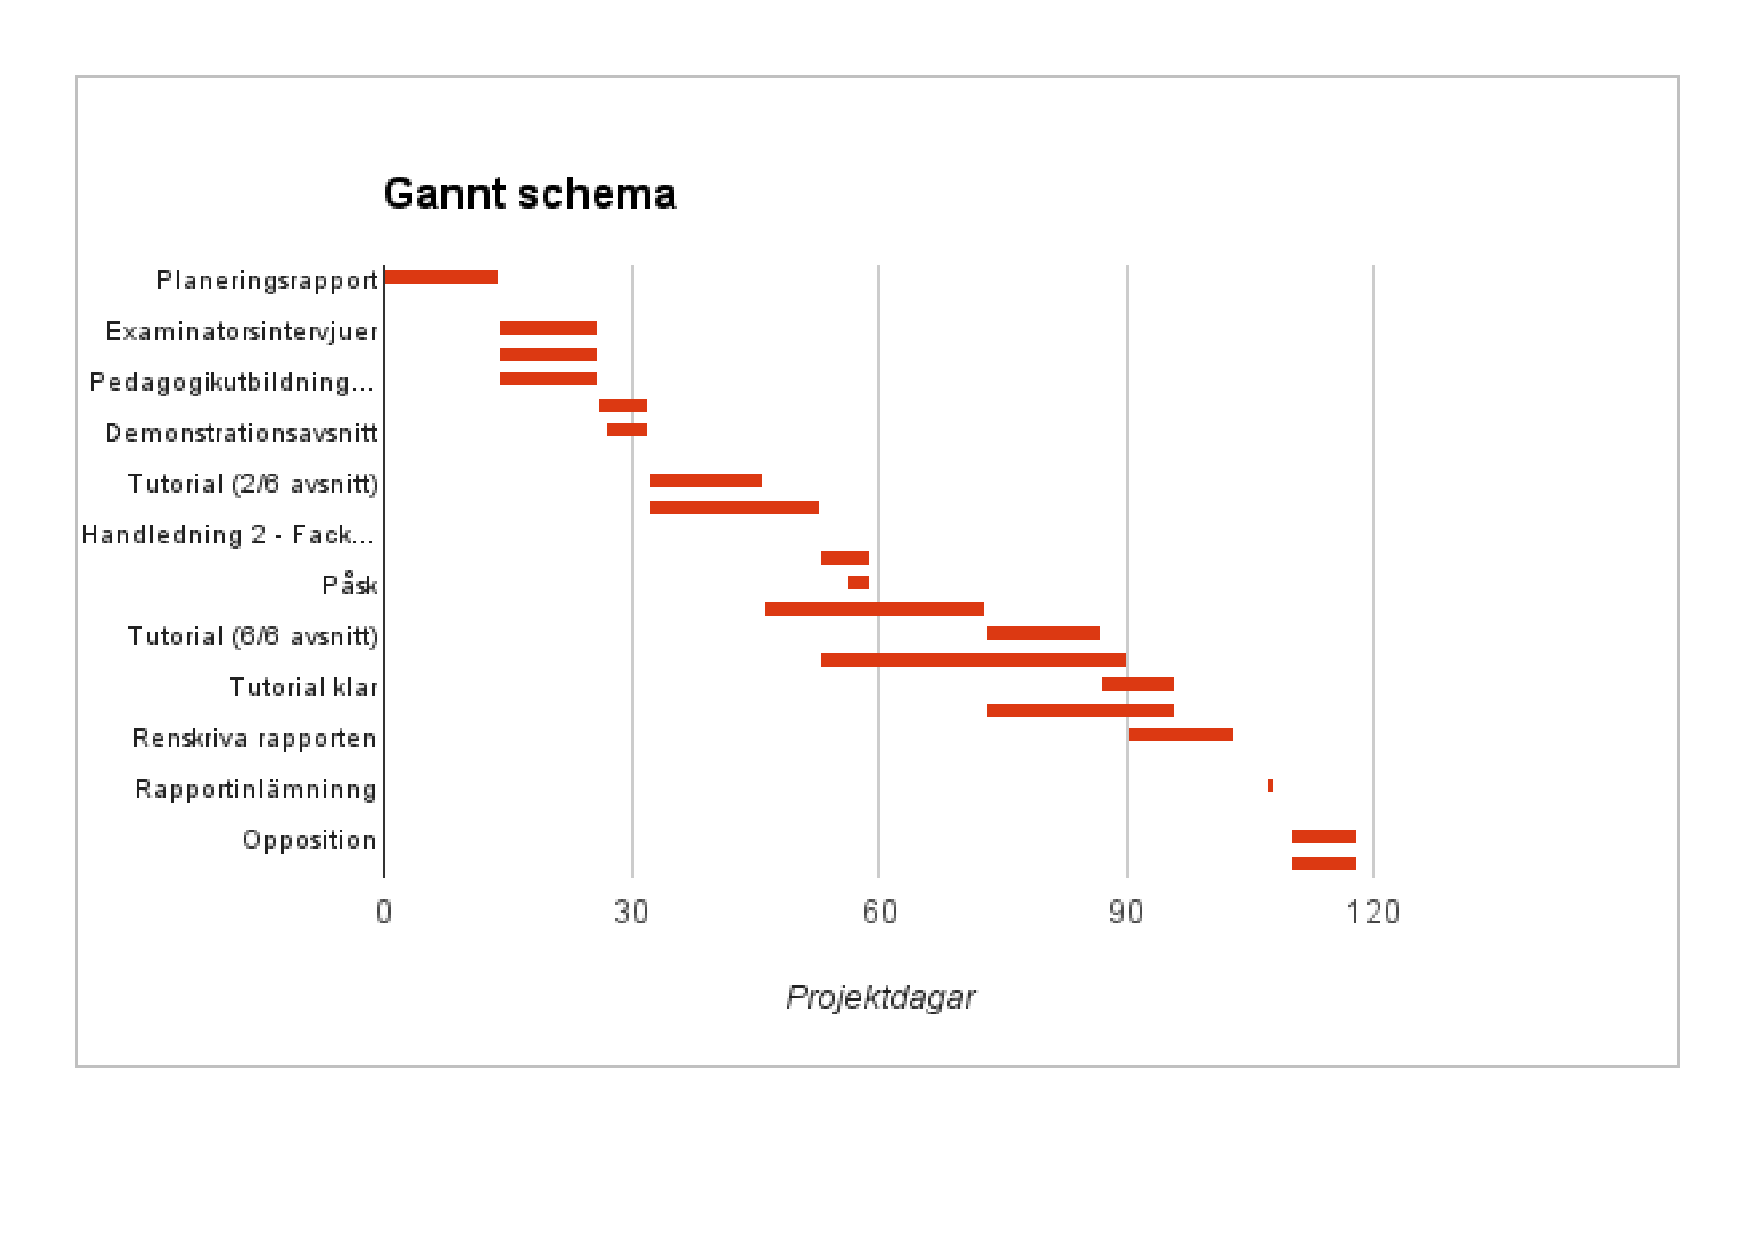
\includepdf[width=0.8\paperwidth]{Gannt}
\end{figure}
\end{document}
